\capitulo{5}{Aspectos relevantes del desarrollo del proyecto}

Este apartado pretende recoger los aspectos más interesantes del desarrollo del proyecto, comentados por los autores del mismo.
Debe incluir desde la exposición del ciclo de vida utilizado, hasta los detalles de mayor relevancia de las fases de análisis, diseño e implementación.

\subsection{Inicio del proyecto}
El tema del proyecto surgió buscando tecnologías que pudieran destacar en un proyecto.

El análisis de sentimiento en texto está muy extendido para los textos en inglés y se nos ocurrió que hacerlo para castellano sería algo destacable.

Además, el uso de redes sociales en los últimos años está muy extendido y utilizarlo en el proyecto podría permitir la recogida de datos muy variados.

Jose Manuel, el tutor, ya había llevado varios proyectos que engloban las redes sociales por lo que era muy útil para dudas en cuanto a la extracción de datos de las APIs. Además de tener varios conocimientos en las series temporales.

Por ello pensamos en una aplicación web que uniera el análisis de sentimiento junto con redes sociales y generación de gráficos y series temporales.

Así fue como surgió la idea de crear la aplicación Sentinel.


\subsection{Metodologías}
La metodología utilizada ha sido SCRUM, metolodología aprendida en la asignatura de gestión de proyectos. Se basa en utilizar la gestión ágil para el proyecto, aunque no se ha seguido estrictamente, sí se han realizado algunos de los eventos que identifican esta metodología.

El desarrollo se ha dividido en sprints, en los cuales se marcaban una serie de objetivos y se estimaba su valor mediante \textit{Story points}. Para esta manera de gestión ha sido muy útil la herramienta Zenhub, la cual nos proporciona un tablero donde podemos interactuar con los distintos estados en los que puede estar una tarea.

En cuanto a las reuniones, se han juntado la reunión de revisión del sprint, retrospectiva del sprint y planificación del sprint. 
Aunque se realizase en una única reunión se seguía el orden de realización.

\begin{itemize}\tightlist
    \item Revisión del sprint: Como su nombre indica se habla de cómo ha ido el sprint, los objetivos que se han conseguido y se muestran los avances.
    \item Retrospectiva del sprint: Se habla de los problemas que se han tenido durante el sprint y lo que sí ha funcionado. Se usa para ver qué aspectos deben cambiar para mejorar la calidad del trabajo.
    \item Planificación del sprint: Al comienzo de cada sprint se habla de los objetivos a conseguir durante ese sprint y la estimación de trabajo que va a llevar cada uno.
    
\end{itemize}

\subsection{Formación}
Para la realización del proyecto se ha necesitado la investigación sobre varios conceptos con los cuales no se habían tratado durante el grado. A continuación se comenta cuáles han sido.

\subsubsection{Sentiment Analysis}
Es el tema principal del proyecto, por lo que era esencial buscar información sobre el tema y conocer cómo funciona.
Para ello se consultaron algunos libros de la biblioteca de la universidad online y varias webs. 

Se buscaron librerías que realizaran los análisis y explicaran qué criterios seguían a la hora de hacerlo.

\subsubsection{Flask}
Para crear la aplicación se utilizó el framework flask, ya que es muy sencillo de utilizar y de instalar. 
Permite crear un servidor en Python de forma rápida y favorece el patrón de diseño de MVC, ya que podemos diferenciar bien las partes del modelo, vista y controlador.

Se contempló la opción de utilizar Django, el cual nos brinda la misma funcionalidad que flask pero está orientado a proyectos más grandes.

\subsubsection{Angular}
Para el desarrollo del Frontend se pensó que era interesante añadir el framework angular.

Como no se había aprendido durante el grado ha sido bastante difícil su aprendizaje, pero gracias a la web de Angular, \url{https://angular.io/}, que ofrece varios ejemplos con el paso a paso, se consiguió aprender cómo realizar servicios y sus comunicaciones con el Back end.

\subsubsection{Series temporales} \cite{time_series_book}
Además de los gráficos que muestran los datos almacenados, se ha decidido introducir series temporales.
Para el aprendizaje, los tutores han proporcionado un curso sobre estas que se impartió para ellos en la UBU, tanto en lenguaje R como en Python.

Además del curso, también han proporcionado una serie de PDFs que permiten la comprensión y el aprendizaje de las series a nivel teórico.

\subsection{Desarrollo del proyecto}
Durante las primeras semanas se eligió el entorno de desarrollo, se investigó sobre trabajos relacionados, sobre flask, el editor de textos para la memoria, etc. 

Tras esto, había que extraer los datos de las APIs, generar el prototipo de la interfaz para la aplicación, conectar nuestra aplicación con la base de datos, conectar flask con angular.
\begin{figure}[h]
    \centering
    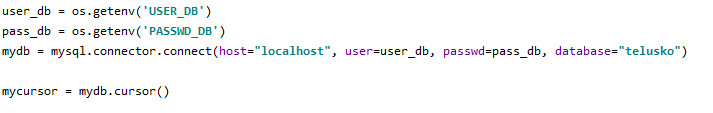
\includegraphics[scale=0.8]{conexionBD}
    \caption{Conexión desde Python con MySQL.}
    \label{fig:my_label}
\end{figure}
\imagen{conexionBD}{Conexión desde Python con MySQL.}

Realizadas todas las conexiones necesarias, se comenzó a buscar sobre librerías de sentiment analysis y como sería su integración con el proyecto.

Mientras, se escogió el template para angular y se ajustó a la aplicación. Después se eligió el segundo template, el de gráficos y se integró con el resto de la aplicación.

\imagen{manual_usuario/inicioES}{Página de inicio de la aplicación.}

Tras haber realizado los métodos de cálculo de análisis, se realizaron los cálculos estádisticos para almacenarlos en una nueva tabla en la base de datos.

\imagen{manual_usuario/tablaEstadisticasES}{Cálculos estadísticos.}

Teniendo ya la parte back end con los cálculos realizados y el front end con los templates bien integrados se comenzó a implementar varias funcionalidades como la de login o la del registro, y una de las principales, la visualización de los resultados en gráficos. 

\imagen{graficosR}{Gráficos implementados.}

Para ello fue necesario aprender a realizar peticiones desde la interfaz al servidor y saber formar el json correctamente en el servidor para que la información enviada fuera accesible.

\imagen{serviciotw}{Servicio de twitter.}
\begin{figure}[h]
    \centering
    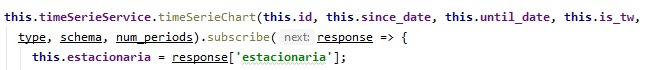
\includegraphics[scale=0.6]{response}
    \caption{Acceso a la información enviada del servidor a la interfaz.}
    \label{fig:my_label}
\end{figure}
\newpage
Además, se implementó la posibilidad de elegir entre qué fechas se quieren mostrar los resultados.
\begin{figure}[!h]
    \centering
    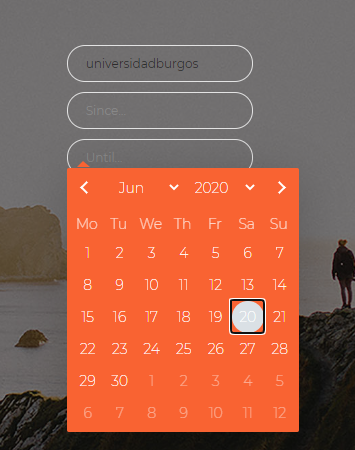
\includegraphics[scale=0.6]{manual_usuario/selectDate}
    \caption{Filtrar por fecha.}
    \label{fig:my_label}
\end{figure}
\FloatBarrier
Hasta el momento los resultados que se podían mostrar estaban previamente guardados, por lo que se añadió la opción de que aunque el identificador buscado no se encuentre en base de datos se busque en las APIs, se guarde en base de datos y se muestren los resultados.
\begin{figure}[h]
    \centering
    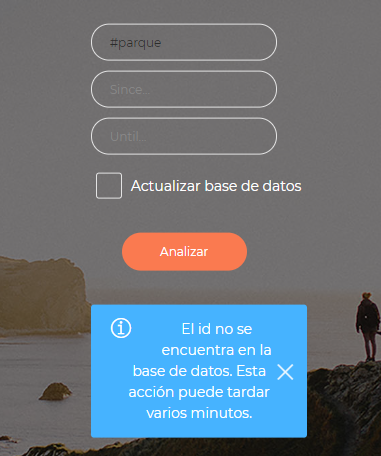
\includegraphics[scale=0.55]{manual_usuario/noIDES}
    \caption{Funcionalidad para buscar un id que no está en la base de datos.}
    \label{fig:my_label}
\end{figure}
\FloatBarrier

Además se añadió la opción de actualizar los identificadores que ya se encuentra en la base de datos.
\begin{figure}[h]
    \centering
    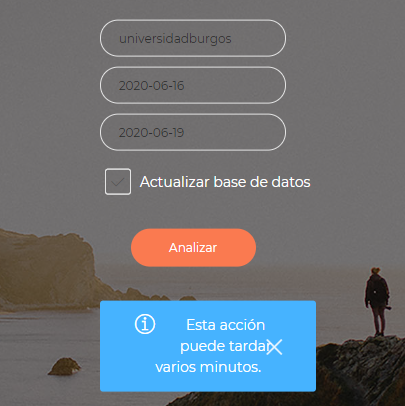
\includegraphics[scale=0.6]{manual_usuario/updateBDES}
    \caption{Funcionalidad para actualizar base de datos.}
    \label{fig:my_label}
\end{figure}
\FloatBarrier

En cuanto a la parte de desarrollo, lo último ha sido la funcionalidad de calcular y mostrar series temporales.

\imagen{manual_usuario/menuTSES}{Menú de elección para el cálculo de series temporales.}

\imagen{manual_usuario/TSgraficoES}{Gráfica de series temporales.}

La última implementación que se ha hecho ha sido la internacionalización, para la cual se han creado dos archivos de extensión json con las traducciones, unas en español y las otras en inglés.
\begin{figure}[h]
    \centering
    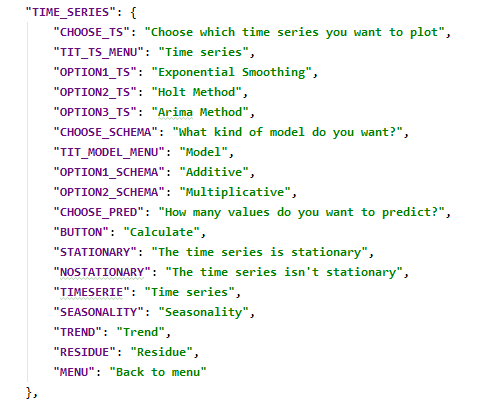
\includegraphics[scale=0.8]{internacionalizacion}
    \caption{Archivo json con las traducciones al inglés.}
    \label{fig:my_label}
\end{figure}

Todas estas implementaciones se han complementado con la documentación sobre el proyecto en memoria y anexos.

\subsection{Resolución de problemas técnicos}
Ha habido algunos problemas a lo largo del desarrollo del proyecto, que se han solventado con éxito.

\subsubsection{Problemas con Angular}

La mayoría de los problemas que se han tenido han sido con Angular ya que es un framework que nunca se había utilizado.

El primer problema fue conseguir ajustar el template de gráficos al template de angular que se ha utilizado para el resto de ventanas. 
Había varios conflictos entre los módulos ya que las versiones no coincidían. Además, algunas de las últimas versiones no son soportadas por estos templates por lo que daba varios errores y no se conseguía levantar la interfaz de usuario.

Ya conseguida la unión de los templates, hubo que aprender a crear servicios y enviar peticiones al servidor y desde este mandar un objeto json bien formado.
Para ello fueron muy útiles los ejemplos con pasos a seguir de la web de Angular como se ha comentado anteriormente.

Para la creación de los gráficos, ha sido necesario añadir un tiempo de parada entre los distintos servicios porque se solapaban entre ellos lo que resultaba en una petición de datos fallida con un código de error 500.

\subsubsection{Problemas con series temporales}
Inicialmente las series temporales a calcular iban a ser el suavizado exponencial, método de Holt y método de Holt-Winters.

Para realizar los cálculos de series temporales es necesario un periodo, el nuestro ha tenido que ser 1 ya que los datos se recogen y almacenan basándonos en el día en el que se crearon. Por ello, los periodos que tendrían sentido serían el 1 o el 7. 
Por ello, se creó un desplegable para que el usuario pudiera escoger entre los dos valores. Pero, al realizar cálculos con el periodo 7 la descomposición de la serie temporal no se realizaba correctamente en ningún caso, por lo que se optó por tener un periodo de 1 siempre.

El problema de tener este valor como periodo, es que el método de Holt-Winters no se podía calcular ya que al ser los valores de análisis tan pequeños, se generaban valores no reales que no se podían representar.
Por ello, decidimos eliminar esta serie temporal.

Pero en su lugar implementamos el modelo Arima, el cual es mucho más complejo y nos permite realizar predicciones más reales.

\subsubsection{Problemas con Heroku}

Para la presentación de la aplicación se decidió desplegar en Heroku, que es un hosting gratuito donde se puede alojar tu página web.
Hubo varios problemas desde el principio ya que el proyecto tiene dos partes, la parte del servidor en la que se realizan todas las operaciones y la interfaz de usuario.
Como están escritas en diferentes lenguajes fue necesario separar las partes para que Heroku pudiera reconocer ambas.
Tras conseguir esto, hubo que modificar algunas partes del código, como las URLs a las que se envían las peticiones, ya que apuntaban al Localhost y ya no iba a corresponder.

Cuando se realizaron las pruebas para ver que todo funcionaba correctamente, se notó la lentitud de la aplicación, pero al ser un hosting gratuito es normal ya que no nos ofrecen mucha memoria.

La aplicación funciona, pero al tener tantos servicios con peticiones agotamos la memoria RAM que nos ofrece Heroku y el rendimiento de la aplicación no es el esperado.

Para poder tener un buen rendimiento, sería necesario pagar una licencia que podría ascender a 250\EUR{}.

Por ello se ha optado por crear una máquina virtual en la que el tribunal pueda realizar las pruebas que considere con un rendimiento óptimo.

\subsubsection{Problemas con la máquina virtual}

Como se ha indicado en el apartado anterior, se ha considerado presentar el proyecto tanto en heroku como en una máquina virtual.
Inicialmente se creó una de Ubuntu, pero al empezar a instalar las dependencias se hizo imposible ya que daban fallos.

Se siguió con una Windows 7, la cual no nos permitió tampoco ya que indicaba que el sistema operativo estaba desactualizado para la version de Visual C++ Tools, las cuales son necesarias para las librerías de análisis de Python.

Por lo cual la solución ha sido comprar una licencia OEM Windows 10 Pro. Con esta se ha conseguido instalar todas las dependencias sin problema y tener la máquina virtual operativa.

Si no se ejecuta la máquina virtual en un ordenador lo suficientemente potente la aplicación puede sufrir fallos de llenado de memoria RAM, como sucedía en Heroku.